\documentclass{article}
\usepackage[final]{nips_2018}
\usepackage[utf8]{inputenc} % allow utf-8 input
\usepackage[T1]{fontenc}    % use 8-bit T1 fonts
\usepackage{hyperref}       % hyperlinks
\usepackage{url}            % simple URL typesetting
\usepackage{booktabs}       % professional-quality tables
\usepackage{amsfonts}       % blackboard math symbols
\usepackage{nicefrac}       % compact symbols for 1/2, etc.
\usepackage{microtype}      % microtypography
\usepackage{amsmath}
\usepackage{amssymb}
\usepackage[mathscr]{euscript}
\usepackage{algorithm}
\usepackage{float}
\usepackage{algorithmic}
\usepackage{graphicx}
\usepackage{calc}
\usepackage{natbib}
\usepackage{subfigure}
\newlength{\depthofsumsign}
\setlength{\depthofsumsign}{\depthof{$\sum$}}
\newlength{\totalheightofsumsign}
\newlength{\heightanddepthofargument}

\DeclareMathOperator*{\argmax}{arg\,max\,}
\DeclareMathOperator*{\argmin}{arg\,min\,}

\title{Recommender system with serendipity}
\author{
  Cl\'{e}mence~R\'{e}da\\
  \'{E}cole Normale Supérieure~Paris-Saclay\\
  supervised by Claire Vernade\\
}


\begin{document}
%\nocite{*}

\maketitle

\begin{abstract}
A lacking feature of current recommender systems is that they usually do not allow discovery of new elements, that is, an element that might be interesting, but which is different of what the user is \textit{used to}. This feature is subject to active research in the domain since 2001, because diversity of recommendation (in a general sense) might be useful in order to avoid overfitting or bias, or boredom of the user. Although the subject of diversity/discovery/... in recommender systems is not new, to the best of my knowledge, there is no formal definition of \textit{serendipity} (that is, a surprisingly good discovery) in the context of recommender systems. The goal of this project was (1) to formalize the problem of recommendation allowing serendipities; (2) to design a method which solves this problem in an online setting; (3) to evaluate its relevance with respect to naive and classic bandit models.
\end{abstract}

\section{Introduction}

Recommender systems have a wide range of applications, from e-commerce (\cite{smith2017two}) to educational data mining (\cite{tang2003smart}). This may account for the high research activity in this field since the early 1980s, and many sorts of methods were developed (see \cite{adomavicius2005toward} for a comprehensive survey of early algorithms). Many researchers (\cite{abbassi2009getting,kunaver2017diversity,zhou2010solving}) have already stressed the difference between \textit{accurate} recommendations (that is, the user actually enjoys the recommended item, and buys it or rates it positively), and \textit{useful} recommendations (recommended items which are novelties, discoveries to the user things that they would never had found themselves). If a recommender system for e-commerce suggests popular items, for instance, most of the users might buy them, but, on the one hand, more obscure books, for instance, might be ignored, thus might never be sold, even if there are users who would be interested in buying them; on the other hand, there might be a drop in sales once the fad for a given item is over, or when most of the customers had already acquired it. The need for diversification of recommender systems is thus strong, and has been a subject of research since 2001 (\cite{bradley2001improving}) (see \cite{kunaver2017diversity} for a recent survey of this sub-field).

This "diversity-accuracy dilemma of recommender systems" (\cite{zhou2010solving}) bears more than a passing resemblance to the exploration-exploitation dilemma that is notably observed in the multi-armed bandit problem (\cite{auer2002finite}). In this project, we will adapt a multi-armed bandit method for Online Influence Maximization to the problem of recommendation with serendipity, and analyze the results with respect to accuracy and diversity.

\section{Problem of Recommendation With Serendipity}

Serendipities are objects that are unexpectedly enjoyable. Two users' reaction to a same recommended item can be poles apart. Thus the difference between serendipity and diversity (\cite{abbassi2009getting}) should be emphasized: diversity is meant to be strictly about recommended object dissimilarity, whereas the notion of serendipity also implicitly depends on the user's past behaviour. More formally, diversity can be quantified by the following measure (\cite{vie2016modeles}):

\begin{equation}
\begin{split}
D(V^{(t)}) & = \sqrt{|V^{(t)}.t(V^{(t)})|}\\
& \mbox{(where $t$ is the number of rounds, $V^{(t)}$ is the matrix which lines are the feature vectors}\\
& \mbox{of explored objects up to time $t$, and $t(V^{(t)})$ its transpose matrix)}\\
\end{split}
\end{equation}

\citet{abbassi2009getting} suggests a definition for $\mathscr{O}\mathscr{B}\mathscr{T}$-ness (\textit{outside-the-box} recommendations), which seems to be an equivalent of the definition of serendipity described above. It relies on a mixture of object and user similarity, and needs offline, fully built user and object similarity networks, along with a few custom parameters which meanings are not straightforward to grasp.

I suggest a definition of serendipity which only relies on:
\begin{enumerate} 
\item the unweighted, undirected object similarity graph, denoted $\mathscr{G}(V, E)$, which is accessible and computable at start time, for in the recommender setting the set of objects is fixed and their feature vectors are known.
\item a \textit{serendipity threshold}, denoted $s$, which quantifies the risk run in order to surprise the user (the higher it is, the more regions of the object graph are available for recommendation).
\item the past behaviour (in terms of exploration and reward) of the user $u$ the algorithm makes recommendations to, denoted $(f_{u}, r_{u})$ (I assume I never have to cope with a cold start case, which seems relevant with respect to the fact I can still ask the user a few ratings/rewards on some movies in order to "initialize" its behaviour). $f^{(t)}_u : V \rightarrow \{0,1\}$ is a random vector that indicates exploration of an object by user $u$ (at time $t$) (thus the notion of \textit{support}, that is, the domain on which $f^{(t)}_{u}$ is positive (denoted Supp($f^{(t)}_{u}$)), is well-defined). $r_u : V \rightarrow \mathscr{R} \subset \mathbb{N}$, a random vector of reward by user $u$ of objects in $\mathscr{G}$. The definition does not assume any prior on the vectors $(f_{u}, r_{u})$, but that I have only access to noisy observations of the rewards and (future) exploration of objects by user $u$, and that, for any given $t$, $(f^{(t)}_{u}, r^{(t)}_{u})$ only depends on the past behaviour of user $u$, i.e. on $(f^{(0)}_{u}, r^{(0)}_{u}), (f^{(1)}_{u}, r^{(1)}_{u}), ..., (f^{(t-1)}_{u}, r^{(t-1)}_{u})$. Here, the user features are implicitly described by the distribution of the user behaviour. Note that $(f^{(0)}_{u}, r^{(0)}_{u})$ can be set using the starting ratings.
\end{enumerate}

The set of potential serendipities at time $t$ for user $u$ (with threshold $s$) is denoted $\mathscr{S}^{(t)}_{u,s}$ and described as follows:

\begin{equation}
\begin{split}
\mathscr{S}^{(t)}_{u,s} & = \argmax_{\substack{v \in V-\text{Supp}(f^{(t)}_{u})\\d(v, \text{Supp}(f^{(t)}_{u})) \leq s}} \mathbb{E}_{(f_{u},r_{u})}[ \sum_{v' \in V} [f^{t+1}_{u}(v")-f_{t}-u(v")]r_{u}(v") ]\\ %TODO
\end{split}
\end{equation}

where , , $d$ is the distance measure used to build $G$ and, for any subset $C$ of objects, $d(., C) = \text{min}_{c \in C} d(., c)$, and $s$ the so-called "serendipity threshold".\\

Intuitively, they can be seen as objects, which are not in already explored regions at time $t$ (i.e. in set $V - \text{Supp}(f^{(t)}_{u})$), and which give the greatest increase in the diameter/support of explored regions of the graph, weighted by the known ratings given by the user $u$.

No assumptions made on past behaviour and ratings. But not computable. More general than the previous definition. ratings may depend on user similarity!!

where E is the expectation: exploration and rating of a node are drawn from a random distribution: when an object is recommended, we "make" the user explore the recommended node, and this modifies the exploration/rating distributions (if the user has enjoyed the recommended object, they will most likely be willing to explore the neighbours of this object).
f-u would likely be submodular (a node can be explored only once, thus at a given point in time, the number of explored elements will increase less and less strongly).

\section{Solving the Problem of Recommendation With Serendipity}

Intuitively, what I want is to increase as fast as possible the support of $f_{u}$ while maximizing the expected rewards of objects in the support. This problem remotely looks like Influence Maximization -I want to select the candidates which will give the highest expected spread, the notion of spread here being the expected reward of unexplored neighbours of each candidate. In order to solve the problem in an online setting, I have adapted the method in \cite{lagree2017effective}. \footnote{The idea of seeing the problem of recommendation with serendipity as an influence maximization problem, and adapting the method in \cite{lagree2017effective} is Claire Vernade's. I have designed the adaptation of the method to recommendation with serendipity and implemented it.} The concept of restricting the set of candidates to a number $K$ of objects (with their "supports", i.e. their direct neighbours in the graph) might suit the idea to restrict recommendations to unexplored suitable regions (see Algorithm \ref{candidates} for the candidate selection, and Algorithm \ref{lagree} for the recommender system). For any matrix $A$, $A[a, b]$ means the submatrix restricted to indices/elements in sets $a$ (row) and $b$ (column), with possibly $a$ or $b$ reduced to a single element.

\begin{algorithm}
\begin{algorithmic}
\STATE \textbf{Name} candidate\_selection
\STATE \textbf{Input} $K$: number of candidates in which the recommended item should be selected, $s$: serendipity threshold, $W$: (unweighted, undirected) similarity graph matrix, $n$: total number of objects, $f$: number of features, $F$: object feature matrix of size $n \times f$.
\STATE \textbf{Output} $\text{candidates}$ the set of candidate nodes for recommendation, and $\text{supports}$ the set of neighbouring unexplored nodes for each candidate.
\STATE - $S \leftarrow \text{Supp}(f^{(t)}_{u}) \cap \{c \in V : \exists i, 1 \leq i \leq s, W^{i}[c, \text{Supp}(f^{(t)}_{u})]\textbf{1} > 0 \}$
\STATE - $\text{centroids} \leftarrow \text{Kmeans}(\text{data}=F[S,:],\text{nclusters}=K)$
\STATE - $\text{candidates} \leftarrow \emptyset$
\FOR{$c \in \text{centroids}$}
\STATE - Append $\argmin_{\substack{v \in S}} ||F[v, :]-F[c, :]||^{2}_2$ to $\text{candidates}$
\ENDFOR
\STATE - $\text{supports} \leftarrow \emptyset$
\FOR{$v \in \text{candidates}$}
\STATE - Append $\{v' \in S : W[v,v'] > 0\}$ to $\text{supports}$
\ENDFOR
\end{algorithmic}
\caption{Candidate selection}
\label{candidates}
\end{algorithm}

The candidate selection problem is hard. \citet{lagree2017effective} suggest getting the nodes with the highest degree, or using Max-Cover to find plausible candidates. My idea is to implement serendipity at this point of the method: at time $t$, I apply $K$-means (\emph{a priori}, any clustering method would be fine, as far as I know) to the set of unexplored elements in the graph at distance lesser than $s$ from the support of $f^{(t)}_{u}$, and, for each computed centroid, I select the closest unexplored existing node (in terms of L2-norm) to this centroid. I have used the fact that $W$ is an adjacency matrix for an unweighted, undirected graph, thus, for any integer $k$ and coordinates $i, j$, $W^{k}[i,j]$ is the number of walks (possibly with repeated edges) of length $k$ between nodes $i$ and $j$. It is implicitly assumed that the number of centroid nodes will be far lesser than the number of nodes in the object graph. 

\begin{algorithm}
\begin{algorithmic}
\STATE \textbf{Name} recommend
\STATE \textbf{Input} $N$: the time budget to evaluate which item should be recommended among the candidates, $\text{candidates}, \text{supports}$ the output of function $\text{candidate\_selection}$.
\STATE \textbf{Output} $a$ the recommended item.
\STATE - Apply \cite{lagree2017effective}'s method on $\text{candidates}, \text{supports}$ for $N$ rounds, and compute the spread of each candidate by sampling the reward of each element in its support.
\STATE - $a$ is the candidate which maximizes the "candidate score" computed in (\cite{lagree2017effective}) at round $N$.
\end{algorithmic}
\caption{Adaptation of \cite{lagree2017effective}'s algorithm for Influence Maximization.}
\label{lagree}
\end{algorithm}

\section{Experiments}

I have compared the adaptation of the method described above with LinUCB (described in \cite{chu2011contextual}), a completely random strategy (see Algorithm \ref{random}), and an $\epsilon$-greedy strategy (see Algorithm \ref{greedy}) on the dataset $\text{ml-1m}$ of MovieLens. 

First, I have selected all ratings associated with the input username, and restricted the benchmark to the movies rated at least once by the user (to avoid the issue of missing data).

Then, I have computed the object feature matrix $F$ as a one-hot encoding of the movie genres for each object (i.e. were a movie $i$ to be classified as "Romance" and "Comedy", and the available labels be "Romance", "Comedy", "Thriller", "Drama" -in this order- the resulting feature line $F[i, :]$ would be $1100$).Then I have built the $\text{eps}$-neighbourhood with parameter $\sigma$: first, I have computed the similarity matrix $S$ such that, for two objects $i,j$, $S(i,j) = \text{exp}(\frac{-||F[i,:]-F[j,:]||^{2}_{2}}{\sigma^{2}})$, and then I have used $S$ to built the adjacency matrix $W$ of the unweighted, undirected similarity graph such that, for two objects $i, j$:

\begin{equation}
\begin{split}
W[i, j] & = 1 \mbox{ if $S(i,j) > \text{eps}$}\\
& = 0 \mbox{ otherwise}\\ 
\end{split}
\end{equation}

I have checked that the provided values for $\text{eps}$ and $\sigma^{2}$ had resulted in a connected graph (to avoid having a pair of movies being at infinite distance from each other).

The two measures I have used to compare the different bandit models are:
\begin{enumerate}
\item The cumulative regret, which is defined as follows at time $T$:

\begin{equation}
\begin{split}
R_{T} & = \\ 
\end{split}
\end{equation}

When computing the regret, we also assume that the best "arm" we could use is among the K selected candidates, thus that we do not question the method with which we select the candidates, which is an hypothesis made in the [Lagrée et al., 2017] article.

\item 

This volume should increase more for recommendation with serendipity than for regular recommendation, because recommended objects are supposed to be less correlated.

\end{enumerate}

Both of these measures are actually averaged across $n\_iter$ trajectories.

%TODO use Monte-Carlo estimate in the benchmark

\begin{algorithm}
\begin{algorithmic}
\STATE \textbf{Name} recommend\_random
\STATE \textbf{Input} $n$: number of objects.
\STATE \textbf{Output} $a$ the recommended item.
\STATE - $a \thicksim \mathscr{U}(\{1, 2, ..., n-1, n\})$ (uniform distribution on a discrete set of size $n$).
\end{algorithmic}
\caption{Random strategy.}
\label{random}
\end{algorithm}

\begin{algorithm}
\begin{algorithmic}
\STATE \textbf{Name} recommend\_greedy
\STATE \textbf{Input} $n$: number of objects, $\epsilon$ the probability of playing the random strategy.
\STATE \textbf{Output} $a$ the recommended item.
\STATE - Draw $e \thicksim \mathscr{B}(\epsilon)$ (Bernouilli distribution of parameter $\epsilon$).
\IF{$e = 1$}
\STATE - $a \thicksim \mathscr{U}(\{1, 2, ..., n-1, n\})$
\ELSE
\STATE - $a = \argmax_{b \in V-\text{Supp}(f^{(t)}_{u})} D(V^{t-1}, F[b, :])$ (diversity measure where the feature vector of $b$ is added as the $t^{th}$ line of the observed feature matrix).
\ENDIF
\end{algorithmic}
\caption{$\epsilon$-greedy strategy.}
\label{greedy}
\end{algorithm}

\begin{figure}[H]
  \centering
  \rule[-.5cm]{0cm}{4cm}
  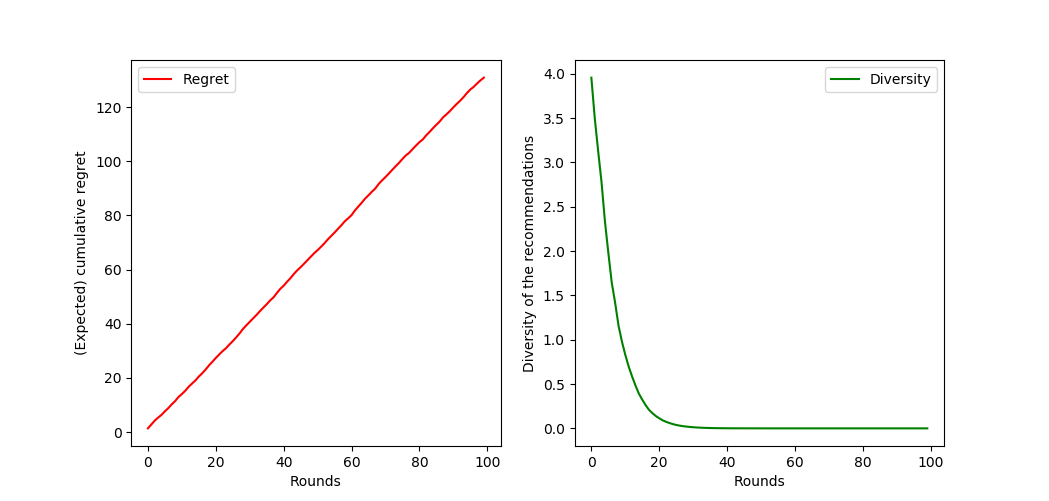
\includegraphics[scale=0.5]{../Results/random_4min40sec.png}
  \rule[-.5cm]{4cm}{0cm}
  \caption{[Random strategy] (Average) cumulative regret and diversity measure over $n\_iter=100$ trajectories, horizon $T=100$, for user $2$ in MovieLens dataset $\text{ml-1m}$. In order to build the $\text{eps}$-neighbourhood similarity graph, I have used values $\text{eps}=0.6$, $\sigma^{2}=100$.}
\end{figure}

\begin{figure}[H]
  \centering
  \rule[-.5cm]{0cm}{4cm}
  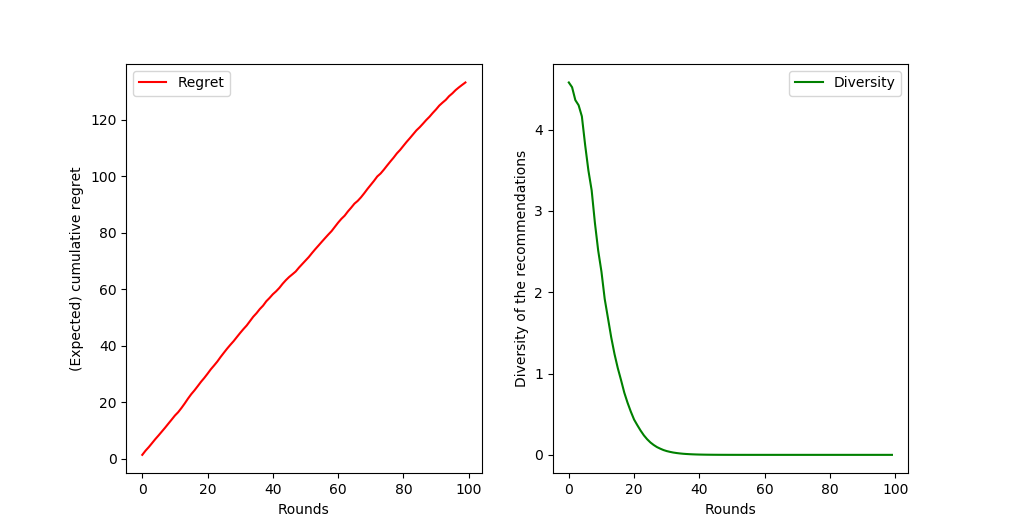
\includegraphics[scale=0.5]{../Results/greedy_51min6sec.png}
  \rule[-.5cm]{4cm}{0cm}
  \caption{[$\epsilon$-greedy strategy] (Average) cumulative regret and diversity measure over $n\_iter=100$ trajectories, horizon $T=100$, for user $2$ in MovieLens dataset $\text{ml-1m}$ and parameter $\epsilon=0.2$. In order to build the $\text{eps}$-neighbourhood similarity graph, I have used values $\text{eps}=0.6$, $\sigma^{2}=100$.}
\end{figure}

\begin{figure}[H]
  \centering
  \rule[-.5cm]{0cm}{4cm}
  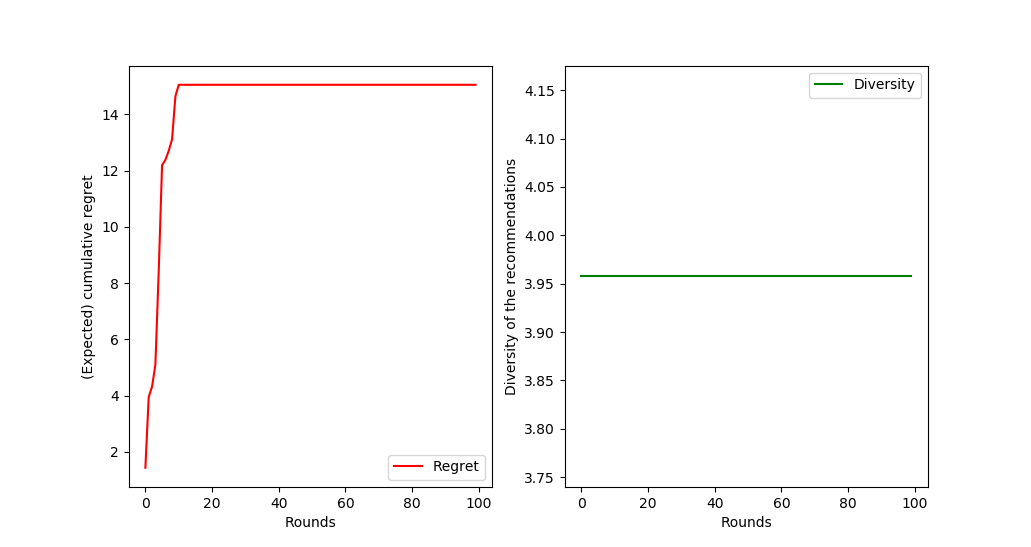
\includegraphics[scale=0.5]{../Results/linUCB_6min4sec.png}
  \rule[-.5cm]{4cm}{0cm}
  \caption{[LinUCB strategy] (Average) cumulative regret and diversity measure over $n\_iter=100$ trajectories, horizon $T=100$, for user $2$ in MovieLens dataset $\text{ml-1m}$ and parameter $\alpha=0.1$. In order to build the $\text{eps}$-neighbourhood similarity graph, I have used values $\text{eps}=0.6$, $\sigma^{2}=100$.}
\end{figure}

\begin{figure}[H]
  \centering
  \rule[-.5cm]{0cm}{4cm}
  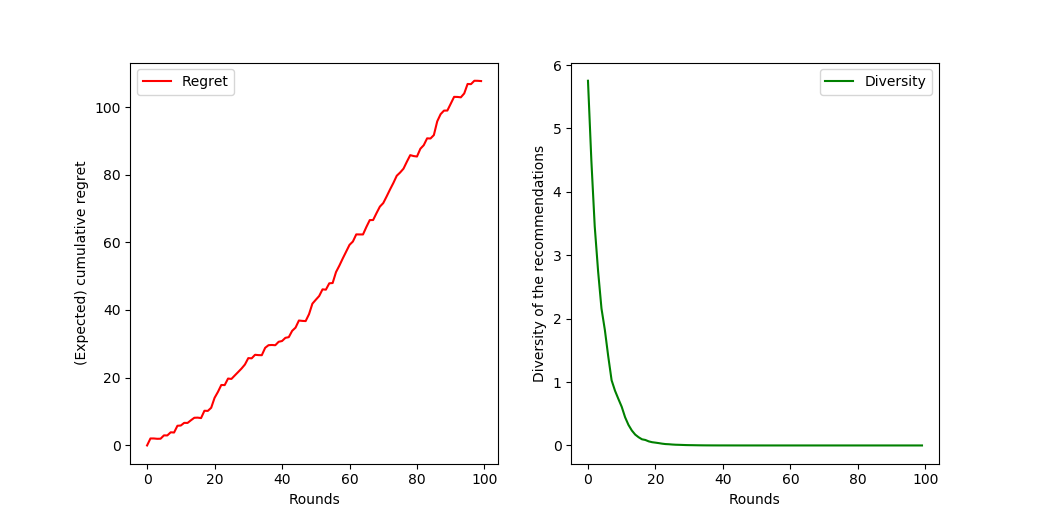
\includegraphics[scale=0.5]{../Results/lagree_36min16sec.png}
  \rule[-.5cm]{4cm}{0cm}
  \caption{[Adapted method strategy] (Average) cumulative regret and diversity measure over $n\_iter=100$ trajectories, horizon $T=100$, for user $2$ in MovieLens dataset $\text{ml-1m}$ and parameter $K=5, s=1, N=10$. In order to build the $\text{eps}$-neighbourhood similarity graph, I have used values $\text{eps}=0.6$, $\sigma^{2}=100$.}
\end{figure}

\begin{figure}[H]
  \centering
  \rule[-.5cm]{0cm}{4cm}
  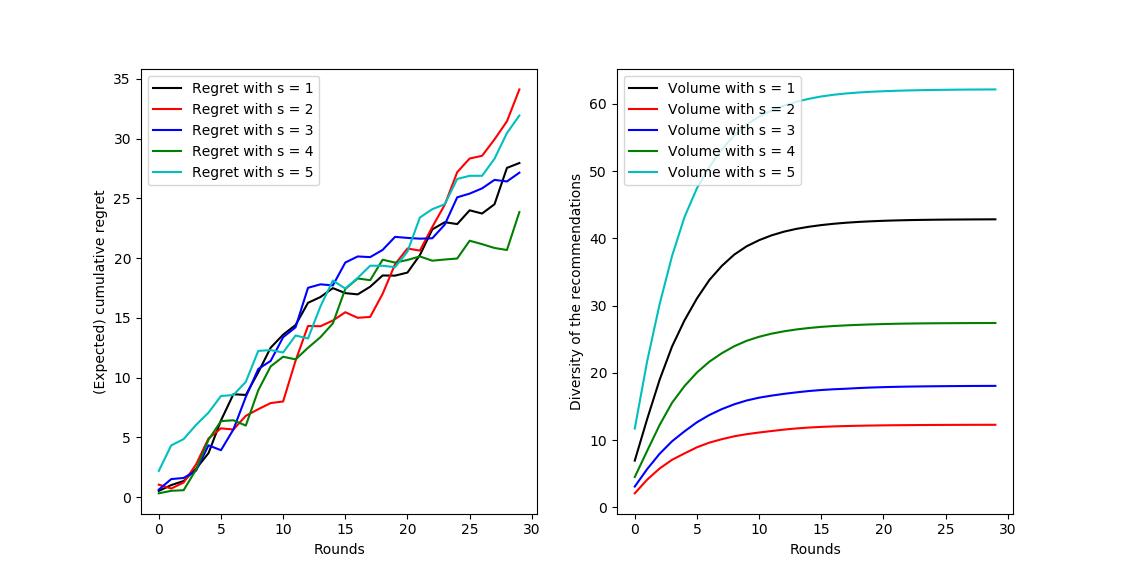
\includegraphics[scale=0.5]{../Results/lagree.png}
  \rule[-.5cm]{4cm}{0cm}
  \caption{[Adapted method strategy] (Average) cumulative regret and diversity measure over $n\_iter=100$ trajectories, horizon $T=100$, for user $2$ in MovieLens dataset $\text{ml-1m}$ and parameter $K=5, N=10$ with varying parameter $s=1, 2, 3, 4, 5$. In order to build the $\text{eps}$-neighbourhood similarity graph, I have used values $\text{eps}=0.6$, $\sigma^{2}=100$.}
\end{figure}

\begin{table}[H]
  \caption{Run times for $n\_iter=100$, horizon $T=100$ for each method.}
  \label{runtimes}
  \centering
  \begin{tabular}{lll}
    \multicolumn{2}{c}{}                   \\
    \cmidrule(r){1-2}
    Method     & Run time    \\
    \midrule
    random & 4 min. 40 sec.  \\
    $\epsilon$-greedy & 51 min. 6 sec.  \\
    LinUCB     & 6 min. 4 sec. \\
    Adapted method     & 36 min. 16 sec.       \\
    \bottomrule
  \end{tabular}
\end{table}

Note that the runtimes listed in Table \ref{runtimes} use Python implementations of each bandit model; coding them in C++ instead would have probably made everything faster. The code itself is not really optimized either, and this may account for the slowness of $\epsilon$-greedy and the adapted method.

\section{Discussion}

%\subsubsection*{Acknowledgments} TODO
%Many thanks to Claire Vernade for mentoring me.

\bibliographystyle{plainnat}
\bibliography{biblio}

\end{document}
